\begin{document}
Pel que fa a l'anàlisis de costos, un dels principals objectius del projecte, s'ha intentat segregar segons els diferents paràmetres on el sistema es pot derivar, que són:
\begin{itemize}
	\item La mida del sistema agregat, és a dir, el nombre de comptadors d'un barri.
	\item L'algorisme emprat per tal de realitzar el logaritme discret.
\end{itemize}
No obstant això, anteriorment s'ha especificat certes propietats que comporta el sistema:
\begin{itemize}
	\item Es considera que entre ronda i ronda passaran hi haurà, com a mínim, un interval de 15 minuts.
	\item El valor màxim que pot enviar un comptador a una subestació en una ronda és, tenint en compte que serà el valor acumulat ronda i una altra.
\item Tenint en compte que en un nucli familiar de 3 persones, hi ha un consum mitjà de $2703 \ \ kWh \; / \; any$, es considerarà que el valor mitjà de lectura dels comptadors intel·ligents serà:
\[\mu = 3272 \ \ \frac{kWh}{any} \cdot \frac{1000 \ Wh}{1 \ kWh} \cdot \frac{1 \ any}{365 \ dies} \cdot \frac{1 \ dia}{24 \ h} = 77,1404\frac{Wh}{h} = 93,3789 \frac{Wh}{15 \ min} \]
A més a més, el conjunt de lectures del sistema agregat en una ronda seguirà una distribució normal, sent el valor central, el consum mitjà $\mu = 93,3789$ i la una desviació estàndard $\sigma = 50 \frac{Wh}{15 min}$, per tal de realitzar una simulació més real a l'hora d'analitzar el límit del sistema.
\begin{figure}[H]
	\centering
	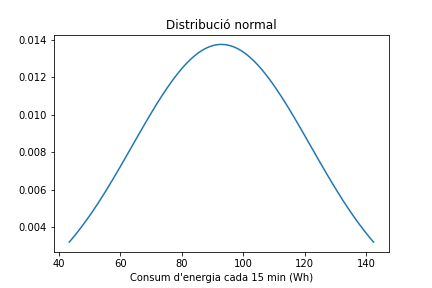
\includegraphics[width=10cm]{imgs/cost/normal.png}
	\caption{Distribució normal}
	\label{fig:normal-dist}
\end{figure}
\end{itemize}
\section{Algorismes de computació del logaritme discret}
El primer que es voldrà analitzar seran els diferents algoritmes implementats que realitzen el logaritme discret, que són un total de tres:
\begin{itemize}
	\item Pollard's Lambda, descrit a la
	\item Algoritme de força bruta \texttt{BruteForce}, que recorre tot el grup per trobar el possible valor.
	\item Algoritme \textit{singleton} de força bruta \texttt{HashedAlgorithm}, on es realitza un cop l'algoritme per guardar les relacions entre els elements i la seva respectiva potència.
\end{itemize}

\section{Comparació entre diferents barris}
\end{document}